\section{Normal Distribution}\label{section:normal-distribution}
In this section, the theory needed to use normal distributions is presented and explained, and has primarily been based on \citet{article:Lauritzen, article:thiesson}.

A normal distribution is common when working with continuous variables \citep{misc:artificial-intelligence}. 
It is a distribution that can be specified by giving the mean and variance, the uncertainty about the expected value of the distribution, notated as $\mathcal{N}(\mu, \sigma^2)$. 
It could be a distribution for the expected result of i.e. acceleration, velocity, or position.

The theory of univariate and multivariate normal distributions is described hereafter, where univariate is for a variable influenced by one factor, whereas multivariate is by multiple factors. 

\subsection{Univariate}
The actual function for a univariate normal distribution is as follows:

\begin{equation}\label{eq:normaldist}
	f(x) = \frac{1}{\sigma \sqrt{2\pi}}e^{-\frac{(x - \mu)^2}{2 * \sigma^2}}
\end{equation}
where, 
\begin{itemize}
	\item[$\mu$] is the mean value of the data. It gives the position of the normal distribution, which is approximated by using $\mu = \frac{1}{n}\sum\limits_{n}\left(X_n\right)	$.
	\item[$\sigma$] is the standard deviation. It is a measurement for the variance of the data, and determines how flat the normal distribution is. $\sigma ^2$ is the variance that is approximated by using $\sigma^2 = \frac{1}{n}\sum\limits_{n}\left( X_n - \mu \right)^2$.
\end{itemize}

\begin{figure}[h]
	\centering
	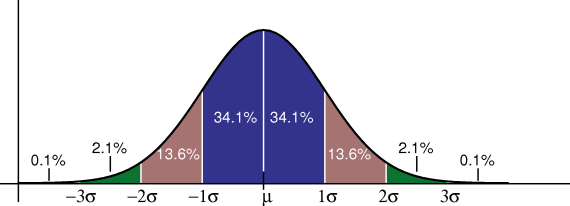
\includegraphics[scale=2]{media/Theory/stddev}
	\caption{Normal distribution \citep{book:gaussian}.}
	\label{fig:stddev}
\end{figure}

To have an idea of how a normal distribution looks, see \figref{fig:stddev}. The figure indicates how the probability is distributed around $\mu$, where $68\%$ of the values is in the range of $\mu \pm \sigma$.
If the integral is taken from $-\infty$ to $\infty$, it will result in $100\%$.

\subsection{Multivariate}
To update the probability distributions for the given variables in the Bayesian network, for each timeslice, it is necessary to have some general theory for joining and marginalisations of probabilities.

The probability distribution for a stochastic vector $X$, where the distribution is normal and not affected by other variable distributions, is defined as follows.
\begin{equation}\label{eq:normaldistindependent}
p(X)=\mathcal{N}(A, C)
\end{equation}

As can be seen in \eqref{eq:normaldistindependent}, the mean value is solely based on $A$, which is a $\begin{bmatrix}a \times b\end{bmatrix}$ matrix.
%For acceleration  in this project it would be the recorded acceleration value, since for acceleration in 1 axis $a = 1$. 
Furthermore, $C$ is a $\begin{bmatrix}a \times a\end{bmatrix}$ co-variance matrix for the normal distribution of $X$. 

When a stochastic vector $Y$ is affected by another stochastic vector $X$, then the conditional density for $Y$ given $X$ is defined as follows. 
\begin{equation}\label{eq:normaldistaffected}
p(Y|X)=\mathcal{N}(E + F * A, G)
\end{equation}

In \eqref{eq:normaldistaffected}, $E + F * A$ can be seen and is a linear regression on $A$.
$E$ is a $\begin{bmatrix}1 \times d\end{bmatrix}$ gain matrix that can be defined, for example if there is a tendency to get a mean value that is always $0.1$ lower than the actual value, $E$ could be $0.1$ to take this into account.
$A$ is a $\begin{bmatrix}c \times d \end{bmatrix}$ matrix, containing the mean values of the parent variables of the affected variable, where $Y$ is the child.
$F$ in this case is a $\begin{bmatrix}1 \times c\end{bmatrix}$ matrix, and is defined such that it correctly describes how $X$ affects the mean value for $Y$, which varies depending on how $X$ is constructed. 
That is, how the different elements of $A$, which are based on the mean values of $X$, affect the mean value of $Y$.
$G$ is the cardinal covariance matrix, for $Y$ given $X$, which for this project has not been determined accurately.
Utilising machine learning techniques, could be helpful to determine the accurate $G$. 

\subsection{Direct Combination}\label{section:direct-combination}
The equation to calculate the joint distribution of $Y$ and $X$ is as follows:
\begin{equation}\label{eq:jointdist}
\begin{aligned}
P(Y,X)&=P(Y|X)*P(X)=\mathcal{N}(U+V,W)\\
U&= 
\begin{bmatrix}
\mu_X \\
\mu_Y 
\end{bmatrix}
= \begin{bmatrix}
A \\
E + F * A
\end{bmatrix}\\
V &= 0\\
W &=
\begin{bmatrix}
\Sigma_{XX} & \Sigma_{XY} \\
\Sigma_{YX} & \Sigma_{YY}
\end{bmatrix}
=
\begin{bmatrix}
C & C * F^\intercal \\
F*C & G + F * C * F^\intercal
\end{bmatrix}
\end{aligned}
\end{equation}

As can be seen in \eqref{eq:jointdist}, $U$ consist of the mean values of $X$ and $Y$.
When $P(X)$ and $P(Y|X)$ have been defined, the partial result can directly be used for $U$.
No additional gain other than $U$ is relevant since $V=0$, as there are no conditional variables in $P(Y,X)$.
The covariance matrix $W$ for $P(Y,X)$ can, as $U$, also be constructed by the partial results of marginalisation $X$ in $P(X)*P(Y|X)$.
The elements of $W$ consists of the variance of $X$ and $Y$ on the diagonal, where the other elements are the co-variances of $X$ and $Y$ combined.
In order to calculate the probability distribution for $Y$, \eqref{eq:marginalised} is used.
\begin{equation}\label{eq:marginalised}
P(Y)=\mathcal{N}(E+F*A,G+F*C*F^\intercal)
\end{equation}

\eqref{eq:marginalised} has been constructed by using $P(Y,X)$, where $X$ has been marginalised out. 
Since the probability distribution, which is being worked with, is a normal distribution, this
marginalisation becomes trivial.
The mean value in the equation is $E+F*A$, since it is the $Y$ part of $U$ in \eqref{eq:jointdist}.
The variance is element $(2,2)$ in $W$ from \eqref{eq:jointdist}.

\subsection{Insertion of Evidence}\label{section:insert-evidence}
When able to calculate the joint distribution of two stochastic variables, it is possible to update the probability distributions with insertion of evidence, which is defined as follows.

\begin{equation}\label{eq:evidence}
\begin{aligned}
P(Y,E) &= \mathcal{N}\left(\begin{bmatrix} A_Y \\ A_E\end{bmatrix}, \begin{bmatrix}C_{YY} & C_{YE} \\ C_{EY} & C_{EE}\end{bmatrix}\right) \\
P(Y,E=e) &= \mathcal{N}\left(U,W\right) \\
U &= A_Y + C_{YE} * (e - A_E) * C_{EE}^{-1} \\
W &= C_{YY} - C_{YE} * C_{EY} * C_{EE}^{-1}
\end{aligned}
\end{equation}

As can be seen in \eqref{eq:evidence}, when evidence is inserted for a stochastic variable, the joint distribution for two variables where one of them has evidence inserted, can be determined from the evidence and the joint distribution of these two variables.

The insertion of evidence theory described above works when having an exact observation. 
However, if an observation is uncertain, the above formulas do not work since the variance from the observation wont have effect on the marginalised distribution of the parent node of the observation.
The theory for evidence can, however, be used in other settings such as the Kalman filter, since in that case the observation is certain.

\subsection{Applying the Formulas}
With the general theory for direct combination described, applying the theory to the Bayesian network for this project can be performed.

See \eqref{eq:accdist} for an example of how to determine the normal distribution of the acceleration.
\begin{equation}\label{eq:accdist}
P(acc_{i+1})=\mathcal{N}(acc_{i+1},\sigma^2_{acc})
\end{equation}

\eqref{eq:accdist} consists of $acc_{i+1}$, which is the recorded data from the accelerometer, and $\sigma^2_{acc}$ is the variance, which is determined in \secref{section:finding-the-variance}. 
The reason the acceleration is represented as a single stochastic node and not as two nodes, where one is the observation of the acceleration and the other is the actual acceleration, is as follows.
As discussed in the previous section about evidence, the variance for the observation would not have an impact on the actual acceleration node. 
For that reason, acceleration has been modelled as a single stochastic node to take the acceleration variance into account for its descendants.

Once this normal distribution is determined, the normal distribution for the moving average of the acceleration $MA_{i+1}$, as seen in \figref{fig:direct-combination}, can be found.

\begin{figure}[H]
\centering
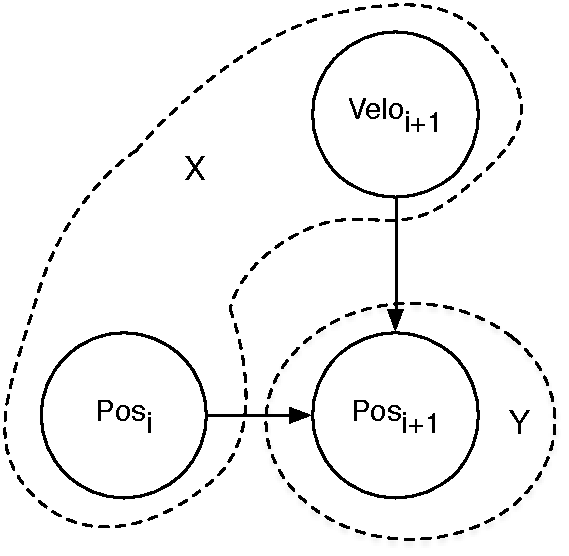
\includegraphics[scale=0.4]{direct-combination}
\caption{A family, or segment, of the Bayesian network from \secref{section:dynamic-bayesian-network}.}
\label{fig:direct-combination}
\end{figure}

With the assumption of a Bayesian network as in \figref{fig:direct-combination}, \eqref{eq:probabilityformovingaverage} is valid, given the previous theory.
\begin{equation}\label{eq:probabilityformovingaverage}
\begin{aligned}
P(Pos_{i+1})&=\mathcal{N}(F_{Pos}*A_{Pos_{i+1}},G_{Pos_{i+1}}+F_{Pos}*C_{Pos_{i+1}}*{F_{Pos}}^\intercal)\\
\text{where}&\\
F_{Pos}&=\begin{bmatrix} \Delta t & 1\end{bmatrix}\\
A_{Pos_{i+1}}&=\begin{bmatrix} \mu(Velo_{i+1}) \\ \mu(Pos_i)\end{bmatrix}\\	
C_{Pos_{i+1}}&=\begin{bmatrix} var(Velo_{i+1}) & 0 \\ 0 & var(Pos_{i}) \end{bmatrix}\\
\end{aligned}
\end{equation}

In \eqref{eq:probabilityformovingaverage}, $F_{Pos}$ is based on the formula for exponential moving average, as seen in \subsecref{subsection:exponential-moving-average}.
$A_{Pos}$ is based on the mean values for the parent variables of $Pos_{i+1}$.
$C$ is a $\begin{bmatrix}2 \times 2\end{bmatrix}$ matrix and is constructed from the variance of the parents.
$G_{Pos_{i+1}}$ is a cardinal covariance matrix for $Pos_{i+1}$ given a stochastic vector consisting of $Velo_{i+1}$ and $Pos_i$.


For a complete set of formulas for the Bayesian network in \secref{section:dynamic-bayesian-network}, derived from the theory in this section, see \appref{app:direct-combination}.
The formulas are excluded from this section as they are derived similar to \eqref{eq:probabilityformovingaverage}.

In principle, to propagate through a family, the process is to first calculate the marginal and conditional distributions and then make a joint distributions for these, whereafter a marginal distribution for the child is found.